% GNUPLOT: LaTeX picture with Postscript
\begingroup
  \makeatletter
  \providecommand\color[2][]{%
    \GenericError{(gnuplot) \space\space\space\@spaces}{%
      Package color not loaded in conjunction with
      terminal option `colourtext'%
    }{See the gnuplot documentation for explanation.%
    }{Either use 'blacktext' in gnuplot or load the package
      color.sty in LaTeX.}%
    \renewcommand\color[2][]{}%
  }%
  \providecommand\includegraphics[2][]{%
    \GenericError{(gnuplot) \space\space\space\@spaces}{%
      Package graphicx or graphics not loaded%
    }{See the gnuplot documentation for explanation.%
    }{The gnuplot epslatex terminal needs graphicx.sty or graphics.sty.}%
    \renewcommand\includegraphics[2][]{}%
  }%
  \providecommand\rotatebox[2]{#2}%
  \@ifundefined{ifGPcolor}{%
    \newif\ifGPcolor
    \GPcolortrue
  }{}%
  \@ifundefined{ifGPblacktext}{%
    \newif\ifGPblacktext
    \GPblacktexttrue
  }{}%
  % define a \g@addto@macro without @ in the name:
  \let\gplgaddtomacro\g@addto@macro
  % define empty templates for all commands taking text:
  \gdef\gplbacktext{}%
  \gdef\gplfronttext{}%
  \makeatother
  \ifGPblacktext
    % no textcolor at all
    \def\colorrgb#1{}%
    \def\colorgray#1{}%
  \else
    % gray or color?
    \ifGPcolor
      \def\colorrgb#1{\color[rgb]{#1}}%
      \def\colorgray#1{\color[gray]{#1}}%
      \expandafter\def\csname LTw\endcsname{\color{white}}%
      \expandafter\def\csname LTb\endcsname{\color{black}}%
      \expandafter\def\csname LTa\endcsname{\color{black}}%
      \expandafter\def\csname LT0\endcsname{\color[rgb]{1,0,0}}%
      \expandafter\def\csname LT1\endcsname{\color[rgb]{0,1,0}}%
      \expandafter\def\csname LT2\endcsname{\color[rgb]{0,0,1}}%
      \expandafter\def\csname LT3\endcsname{\color[rgb]{1,0,1}}%
      \expandafter\def\csname LT4\endcsname{\color[rgb]{0,1,1}}%
      \expandafter\def\csname LT5\endcsname{\color[rgb]{1,1,0}}%
      \expandafter\def\csname LT6\endcsname{\color[rgb]{0,0,0}}%
      \expandafter\def\csname LT7\endcsname{\color[rgb]{1,0.3,0}}%
      \expandafter\def\csname LT8\endcsname{\color[rgb]{0.5,0.5,0.5}}%
    \else
      % gray
      \def\colorrgb#1{\color{black}}%
      \def\colorgray#1{\color[gray]{#1}}%
      \expandafter\def\csname LTw\endcsname{\color{white}}%
      \expandafter\def\csname LTb\endcsname{\color{black}}%
      \expandafter\def\csname LTa\endcsname{\color{black}}%
      \expandafter\def\csname LT0\endcsname{\color{black}}%
      \expandafter\def\csname LT1\endcsname{\color{black}}%
      \expandafter\def\csname LT2\endcsname{\color{black}}%
      \expandafter\def\csname LT3\endcsname{\color{black}}%
      \expandafter\def\csname LT4\endcsname{\color{black}}%
      \expandafter\def\csname LT5\endcsname{\color{black}}%
      \expandafter\def\csname LT6\endcsname{\color{black}}%
      \expandafter\def\csname LT7\endcsname{\color{black}}%
      \expandafter\def\csname LT8\endcsname{\color{black}}%
    \fi
  \fi
  \setlength{\unitlength}{0.0500bp}%
  \begin{picture}(8206.00,11520.00)%
    \gplgaddtomacro\gplbacktext{%
      \csname LTb\endcsname%
      \put(688,8063){\makebox(0,0)[r]{\strut{}0}}%
      \csname LTb\endcsname%
      \put(688,8639){\makebox(0,0)[r]{\strut{}20}}%
      \csname LTb\endcsname%
      \put(688,9215){\makebox(0,0)[r]{\strut{}40}}%
      \csname LTb\endcsname%
      \put(688,9791){\makebox(0,0)[r]{\strut{}60}}%
      \csname LTb\endcsname%
      \put(688,10367){\makebox(0,0)[r]{\strut{}80}}%
      \csname LTb\endcsname%
      \put(688,10943){\makebox(0,0)[r]{\strut{}100}}%
      \csname LTb\endcsname%
      \put(820,7843){\makebox(0,0){\strut{} 0}}%
      \csname LTb\endcsname%
      \put(1299,7843){\makebox(0,0){\strut{} 5}}%
      \csname LTb\endcsname%
      \put(1777,7843){\makebox(0,0){\strut{} 10}}%
      \csname LTb\endcsname%
      \put(2256,7843){\makebox(0,0){\strut{} 15}}%
      \csname LTb\endcsname%
      \put(2735,7843){\makebox(0,0){\strut{} 20}}%
      \csname LTb\endcsname%
      \put(3213,7843){\makebox(0,0){\strut{} 25}}%
      \csname LTb\endcsname%
      \put(3692,7843){\makebox(0,0){\strut{} 30}}%
      \put(50,9503){\rotatebox{-270}{\makebox(0,0){\strut{}Counts}}}%
      \put(2256,7557){\makebox(0,0){\strut{}}}%
      \put(3347,10713){\makebox(0,0)[l]{\strut{}Ag}}%
    }%
    \gplgaddtomacro\gplfronttext{%
    }%
    \gplgaddtomacro\gplbacktext{%
      \csname LTb\endcsname%
      \put(4381,8063){\makebox(0,0)[r]{\strut{}0}}%
      \csname LTb\endcsname%
      \put(4381,8423){\makebox(0,0)[r]{\strut{}500}}%
      \csname LTb\endcsname%
      \put(4381,8783){\makebox(0,0)[r]{\strut{}1000}}%
      \csname LTb\endcsname%
      \put(4381,9143){\makebox(0,0)[r]{\strut{}1500}}%
      \csname LTb\endcsname%
      \put(4381,9503){\makebox(0,0)[r]{\strut{}2000}}%
      \csname LTb\endcsname%
      \put(4381,9863){\makebox(0,0)[r]{\strut{}2500}}%
      \csname LTb\endcsname%
      \put(4381,10223){\makebox(0,0)[r]{\strut{}3000}}%
      \csname LTb\endcsname%
      \put(4381,10583){\makebox(0,0)[r]{\strut{}3500}}%
      \csname LTb\endcsname%
      \put(4381,10943){\makebox(0,0)[r]{\strut{}4000}}%
      \csname LTb\endcsname%
      \put(4513,7843){\makebox(0,0){\strut{} 2}}%
      \csname LTb\endcsname%
      \put(4872,7843){\makebox(0,0){\strut{} 3}}%
      \csname LTb\endcsname%
      \put(5231,7843){\makebox(0,0){\strut{} 4}}%
      \csname LTb\endcsname%
      \put(5590,7843){\makebox(0,0){\strut{} 5}}%
      \csname LTb\endcsname%
      \put(5949,7843){\makebox(0,0){\strut{} 6}}%
      \csname LTb\endcsname%
      \put(6307,7843){\makebox(0,0){\strut{} 7}}%
      \csname LTb\endcsname%
      \put(6666,7843){\makebox(0,0){\strut{} 8}}%
      \csname LTb\endcsname%
      \put(7025,7843){\makebox(0,0){\strut{} 9}}%
      \csname LTb\endcsname%
      \put(7384,7843){\makebox(0,0){\strut{} 10}}%
      \put(5948,7557){\makebox(0,0){\strut{}}}%
      \put(7039,10713){\makebox(0,0)[l]{\strut{}Ti}}%
    }%
    \gplgaddtomacro\gplfronttext{%
    }%
    \gplgaddtomacro\gplbacktext{%
      \csname LTb\endcsname%
      \put(688,4608){\makebox(0,0)[r]{\strut{}0}}%
      \csname LTb\endcsname%
      \put(688,4968){\makebox(0,0)[r]{\strut{}100}}%
      \csname LTb\endcsname%
      \put(688,5328){\makebox(0,0)[r]{\strut{}200}}%
      \csname LTb\endcsname%
      \put(688,5688){\makebox(0,0)[r]{\strut{}300}}%
      \csname LTb\endcsname%
      \put(688,6047){\makebox(0,0)[r]{\strut{}400}}%
      \csname LTb\endcsname%
      \put(688,6407){\makebox(0,0)[r]{\strut{}500}}%
      \csname LTb\endcsname%
      \put(688,6767){\makebox(0,0)[r]{\strut{}600}}%
      \csname LTb\endcsname%
      \put(688,7127){\makebox(0,0)[r]{\strut{}700}}%
      \csname LTb\endcsname%
      \put(688,7487){\makebox(0,0)[r]{\strut{}800}}%
      \csname LTb\endcsname%
      \put(820,4388){\makebox(0,0){\strut{} 4}}%
      \csname LTb\endcsname%
      \put(1394,4388){\makebox(0,0){\strut{} 6}}%
      \csname LTb\endcsname%
      \put(1969,4388){\makebox(0,0){\strut{} 8}}%
      \csname LTb\endcsname%
      \put(2543,4388){\makebox(0,0){\strut{} 10}}%
      \csname LTb\endcsname%
      \put(3118,4388){\makebox(0,0){\strut{} 12}}%
      \csname LTb\endcsname%
      \put(3692,4388){\makebox(0,0){\strut{} 14}}%
      \put(50,6047){\rotatebox{-270}{\makebox(0,0){\strut{}Counts}}}%
      \put(2256,4102){\makebox(0,0){\strut{}}}%
      \put(3347,7257){\makebox(0,0)[l]{\strut{}W}}%
    }%
    \gplgaddtomacro\gplfronttext{%
    }%
    \gplgaddtomacro\gplbacktext{%
      \csname LTb\endcsname%
      \put(4381,4608){\makebox(0,0)[r]{\strut{}0}}%
      \csname LTb\endcsname%
      \put(4381,5184){\makebox(0,0)[r]{\strut{}50}}%
      \csname LTb\endcsname%
      \put(4381,5760){\makebox(0,0)[r]{\strut{}100}}%
      \csname LTb\endcsname%
      \put(4381,6335){\makebox(0,0)[r]{\strut{}150}}%
      \csname LTb\endcsname%
      \put(4381,6911){\makebox(0,0)[r]{\strut{}200}}%
      \csname LTb\endcsname%
      \put(4381,7487){\makebox(0,0)[r]{\strut{}250}}%
      \csname LTb\endcsname%
      \put(4513,4388){\makebox(0,0){\strut{} 0}}%
      \csname LTb\endcsname%
      \put(4992,4388){\makebox(0,0){\strut{} 5}}%
      \csname LTb\endcsname%
      \put(5470,4388){\makebox(0,0){\strut{} 10}}%
      \csname LTb\endcsname%
      \put(5949,4388){\makebox(0,0){\strut{} 15}}%
      \csname LTb\endcsname%
      \put(6427,4388){\makebox(0,0){\strut{} 20}}%
      \csname LTb\endcsname%
      \put(6906,4388){\makebox(0,0){\strut{} 25}}%
      \csname LTb\endcsname%
      \put(7384,4388){\makebox(0,0){\strut{} 30}}%
      \put(5948,4102){\makebox(0,0){\strut{}}}%
      \put(7039,7257){\makebox(0,0)[l]{\strut{}Sn}}%
    }%
    \gplgaddtomacro\gplfronttext{%
    }%
    \gplgaddtomacro\gplbacktext{%
      \csname LTb\endcsname%
      \put(688,1152){\makebox(0,0)[r]{\strut{}0}}%
      \csname LTb\endcsname%
      \put(688,1512){\makebox(0,0)[r]{\strut{}500}}%
      \csname LTb\endcsname%
      \put(688,1872){\makebox(0,0)[r]{\strut{}1000}}%
      \csname LTb\endcsname%
      \put(688,2232){\makebox(0,0)[r]{\strut{}1500}}%
      \csname LTb\endcsname%
      \put(688,2592){\makebox(0,0)[r]{\strut{}2000}}%
      \csname LTb\endcsname%
      \put(688,2951){\makebox(0,0)[r]{\strut{}2500}}%
      \csname LTb\endcsname%
      \put(688,3311){\makebox(0,0)[r]{\strut{}3000}}%
      \csname LTb\endcsname%
      \put(688,3671){\makebox(0,0)[r]{\strut{}3500}}%
      \csname LTb\endcsname%
      \put(688,4031){\makebox(0,0)[r]{\strut{}4000}}%
      \csname LTb\endcsname%
      \put(820,932){\makebox(0,0){\strut{} 5}}%
      \csname LTb\endcsname%
      \put(1299,932){\makebox(0,0){\strut{} 6}}%
      \csname LTb\endcsname%
      \put(1777,932){\makebox(0,0){\strut{} 7}}%
      \csname LTb\endcsname%
      \put(2256,932){\makebox(0,0){\strut{} 8}}%
      \csname LTb\endcsname%
      \put(2735,932){\makebox(0,0){\strut{} 9}}%
      \csname LTb\endcsname%
      \put(3213,932){\makebox(0,0){\strut{} 10}}%
      \csname LTb\endcsname%
      \put(3692,932){\makebox(0,0){\strut{} 11}}%
      \put(-82,2591){\rotatebox{-270}{\makebox(0,0){\strut{}Counts}}}%
      \put(2256,602){\makebox(0,0){\strut{}Energie $E / \si{\kilo\electronvolt}$}}%
      \put(3347,3801){\makebox(0,0)[l]{\strut{}Zn}}%
    }%
    \gplgaddtomacro\gplfronttext{%
    }%
    \gplgaddtomacro\gplbacktext{%
      \csname LTb\endcsname%
      \put(4381,1152){\makebox(0,0)[r]{\strut{}0}}%
      \csname LTb\endcsname%
      \put(4381,1512){\makebox(0,0)[r]{\strut{}100}}%
      \csname LTb\endcsname%
      \put(4381,1872){\makebox(0,0)[r]{\strut{}200}}%
      \csname LTb\endcsname%
      \put(4381,2232){\makebox(0,0)[r]{\strut{}300}}%
      \csname LTb\endcsname%
      \put(4381,2591){\makebox(0,0)[r]{\strut{}400}}%
      \csname LTb\endcsname%
      \put(4381,2951){\makebox(0,0)[r]{\strut{}500}}%
      \csname LTb\endcsname%
      \put(4381,3311){\makebox(0,0)[r]{\strut{}600}}%
      \csname LTb\endcsname%
      \put(4381,3671){\makebox(0,0)[r]{\strut{}700}}%
      \csname LTb\endcsname%
      \put(4381,4031){\makebox(0,0)[r]{\strut{}800}}%
      \csname LTb\endcsname%
      \put(4513,932){\makebox(0,0){\strut{} 0}}%
      \csname LTb\endcsname%
      \put(5231,932){\makebox(0,0){\strut{} 5}}%
      \csname LTb\endcsname%
      \put(5949,932){\makebox(0,0){\strut{} 10}}%
      \csname LTb\endcsname%
      \put(6666,932){\makebox(0,0){\strut{} 15}}%
      \csname LTb\endcsname%
      \put(7384,932){\makebox(0,0){\strut{} 20}}%
      \put(5948,602){\makebox(0,0){\strut{}Energie $E / \si{\kilo\electronvolt}$}}%
      \put(7039,3801){\makebox(0,0)[l]{\strut{}Zr}}%
    }%
    \gplgaddtomacro\gplfronttext{%
    }%
    \gplbacktext
    \put(0,0){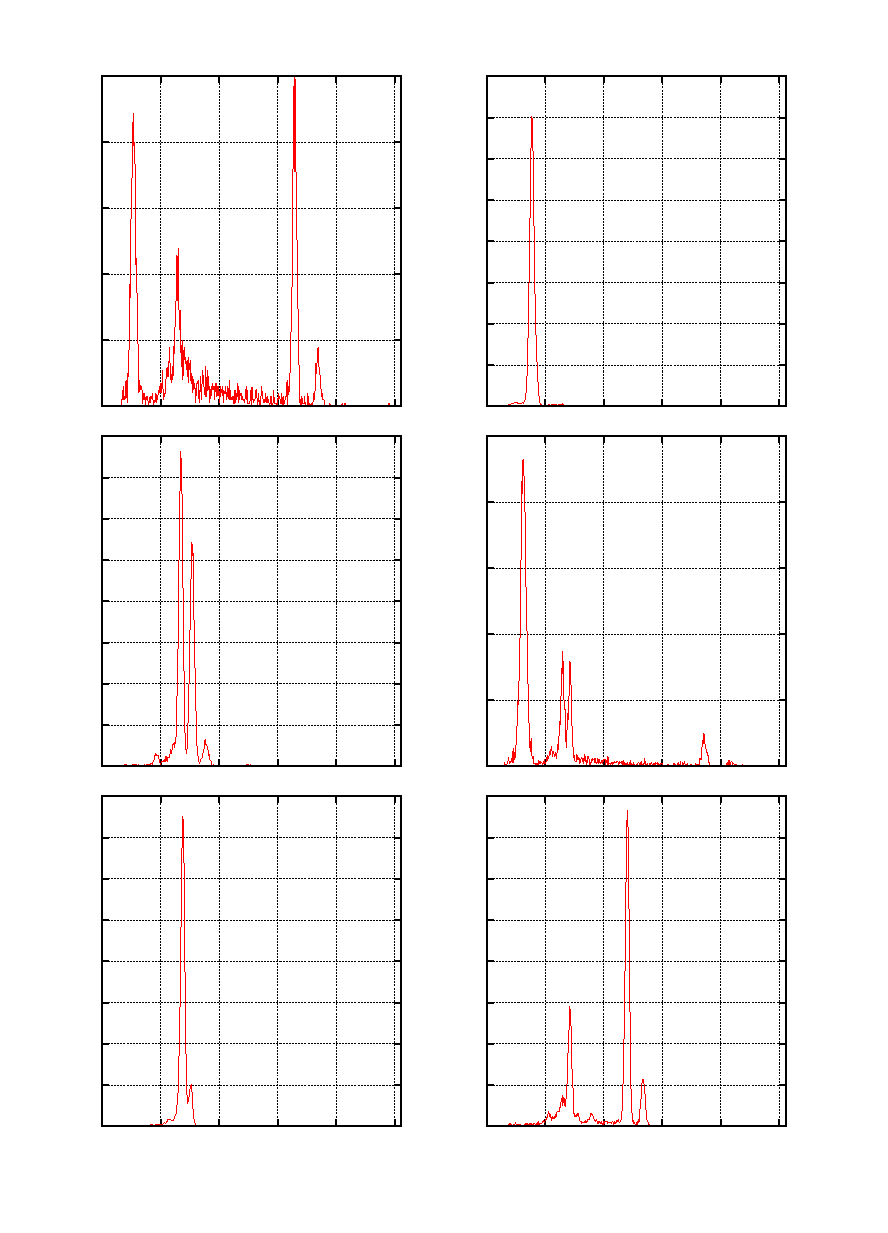
\includegraphics{./plots/referenzspektren2}}%
    \gplfronttext
  \end{picture}%
\endgroup
